\documentclass[rnd]{mas_proposal}
% \documentclass[thesis]{mas_proposal}

\usepackage[utf8]{inputenc}
\usepackage{amsmath}
\usepackage{amsfonts}
\usepackage{amssymb}
\usepackage{graphicx}
\usepackage{pdflscape}

\title{Object detection in adverse weather conditions using tightly-coupled data-driven multimodal sensor fusion}
\author{Kevin Patel}
\supervisors{Prof. Dr.-Ing. Sebastian Houben\\M.Sc. Santosh Thoduka}
\date{February 2023}

% \thirdpartylogo{path/to/your/image}

\begin{document}

\maketitle

\pagestyle{plain}

\section{Introduction}

\subsection{Topic of This R\&D Project}
\begin{itemize}
    % *************************
    % \item Provide reasonably detailed description of what you intent to do in your R\&D project.
    % \item You may also discuss the challenges that you have to address.
    % \item Reflect on the profile of the reader and PLEAAAASE, tell a story here and refrain from bombarding the readers with details which they may not be able to appreciate.
    % **************************

    % \item What is Sensor Fusion?
    % \begin{itemize}
    %     \item The process of combining data from multiple sensors to provide a more accurate, reliable, and comprehensive understanding of an environment or situation.
    % \end{itemize}

    % Why do we need multi-modal sensor fusion?
    % Check where to put this question

    % \item To address this challenge, our research and development project aims to fuse different sensor modalities, including point cloud, pixel, and time series data, to improve perception and object detection accuracy in a variety of adverse weather conditions.

    % \item Fuse different sensor modalities like point cloud, pixels, and time series 
    % \item Improve perception in adverse weather conditions e.g., fog, rain, snow, overcast, sleet, night
    % \item Synchronization of multi-modal data
    % \item Process dense and sparse resolution sensors data
    % \item Make use of a data-driven approach
    % \item Geometrically alignments of different sensors
    % \item Real-time sensor fusion with low latency

    \item Imagine driving on a winding mountain road at night, with fog and rain obscuring your view, your vehicle's self-driving system struggles to detect objects ahead due to the challenging weather conditions. Suddenly, a deer jumps out in front of your car, causing the system to issue an alert and apply the brakes in time to avoid a collision.

    \item This scenario highlights the importance of object detection in adverse weather conditions for self-driving cars. Visual cameras, which are commonly used for object detection, may be distorted or obscured by rain, fog, snow, or low light, making it difficult to accurately detect objects on the road \cite{yurtsever2020survey} \cite{carballo2020libre} \cite{mcity2020}.

    \item To address these challenges, this project aims to implement a multimodal sensor fusion system that combines cameras, radar, and LiDAR sensors. By fusing data from multiple sensors and leveraging advanced machine learning algorithms, the goal is to enhance object detection's range, accuracy, and reliability in adverse weather conditions.

    \item The focus will also be on synchronizing multimodal data, processing dense and sparse resolution sensor data, and using a data-driven approach to optimize object detection performance.

    \item However, this project also faces several challenges. For example, different sensors may have different resolutions and sampling rates and may require sophisticated calibration and alignment techniques to ensure the accurate fusion of their data. Furthermore, processing large volumes of sensor data with minimal latency requires efficient and scalable algorithms and hardware architectures.

    \item The proposed system will be trained on a diverse dataset to ensure robustness and adaptability in different weather and lighting conditions. The system's effectiveness will be evaluated by extensive experiments and by comparing existing state-of-the-art methods.

    \item Despite the challenges, the project has the potential to revolutionize object detection in adverse weather conditions, with applications ranging from self-driving cars to surveillance and security systems. By fusing multiple sensor data sources and optimizing their fusion, situational awareness can be enhanced, enabling safer and more efficient operations in various domains.

    \item This research aims to facilitate safe and efficient self-driving in adverse weather conditions, prioritizing the safety of passengers, other drivers, and pedestrians on the road. To accomplish this, the proposed approach is to develop a sensor fusion system that operates with minimal latency, enabling data processing from multiple sensors in near real-time.

          % write code to put next item on new page
          \newpage

    \item Topic naming convention:
          \begin{itemize}
              \item Object detection
                    \begin{itemize}
                        \item Refers to the task of detecting objects within an image or video stream.
                        \item In this project, the focus is on detecting 2D objects such as cars, trucks, pedestrians, and cyclists.
                    \end{itemize}
              \item Adverse weather conditions
                    \begin{itemize}
                        \item Refers to conditions such as fog, snow, rain, overcast skies, sleet, and dust.
                        \item These conditions can make object detection more challenging due to reduced visibility or other environmental factors.
                    \end{itemize}
              \item Tightly-coupled
                    \begin{itemize}
                        \item Refers to how different modalities of data are combined and integrated at different levels.
                        \item Rather than relying solely on early, mid, or late fusion techniques, a combination of features at different levels is employed to achieve optimal fusion results.
                    \end{itemize}
              \item Data-driven
                    \begin{itemize}
                        \item Refers to the use of previously collected data or publicly available datasets to improve object detection performance.
                    \end{itemize}
              \item Multimodal
                    \begin{itemize}
                        \item Refers to the use of different data modalities to improve object detection performance.
                        \item Examples include sensors such as LiDAR, camera, IMU, GPS, infrared, and radar, with different datatypes such as point clouds, images, and time series data.
                    \end{itemize}
              \item Sensor fusion
                    \begin{itemize}
                        \item Refers to the process of fusing data from different sensors to get a better estimation of an environment and improve object detection performance.
                    \end{itemize}
          \end{itemize}

          % \begin{itemize}
          %     \item {Object detection}
          %     \begin{itemize}
          %         \item 2D object detection - car, truck, pedestrian, cycle
          %     \end{itemize}

          %     \item {Adverse weather conditions}
          %     \begin{itemize}
          %         \item Fog, snow, rainy, overcast, sleet, dust
          %     \end{itemize}

          %     \item {Tightly-coupled}
          %     \begin{itemize}
          %         \item How different modalities are combined at what level
          %         \begin{itemize}
          %             \item Eg. sensor fusion, mid fusion/feature fusion, late fusion, ROI fusion, decision fusion
          %         \end{itemize}
          %     \end{itemize}

          %     \item {Data-driven}
          %     \begin{itemize}
          %         \item Using previously collected data or publicly available datasets
          %     \end{itemize}

          %     \item {Multi-modal}
          %     \begin{itemize}
          %         \item Using different data modalities
          %         \begin{itemize}
          %             \item Sensors: LiDAR, camera, IMU, GPS, infrared, radar
          %             \item Datatypes: Point cloud, image, timer series
          %         \end{itemize}
          %     \end{itemize}

          %     \item {Sensor fusion}
          %     \begin{itemize}
          %         \item Fuse different sensors data to get a better estimation of an environment
          %     \end{itemize}
          % \end{itemize}


\end{itemize}

\subsection{Relevance of This R\&D Project}
\begin{itemize}
    % CAGR - Compound Annual Growth Rate

    \item The relevance of the research project lies in the fact that weather phenomena have a significant negative influence on traffic and transportation, which can lead to accidents, injuries, and fatalities.

    \item The statistics show that adverse weather conditions, such as rain, snow, sleet, and fog, contribute to a high number of vehicle crashes and fatalities worldwide.

    \item For example, in the United States, over 30,000 vehicle crashes occur on snowy or icy roads each year, causing over 5,000 fatalities and 418,000 injuries due to adverse weather-related crashes, according to the Federal Highway Administration (FHA) \cite{federal-highway-administration-no-date} \cite{usDepartmentofCommerce2016}.

    \item The Insurance Institute for Highway Safety (IIHS) found that in snowy weather, the fatal crash rate is 21\% higher than on clear roads, while during sleet and freezing rain, the rate is even higher at 37\%. Moreover, poor visibility is a contributing factor in over 7,000 annual crashes in the United States, according to the FHA, and in over 4,000 fatal crashes in 2018, according to the National Highway Traffic Safety Administration (NHTSA) \cite{brumbelow2022light}.

    \item In Europe, adverse weather conditions cause 25\% of all road accidents, with frost and ice, snow, and rain being the highest contributing factors, according to the European Commission and the European Transport Safety Council (ETSC). Over 12,000 people die on European roads each year in weather-related accidents \cite{cookson-2022}.

    \item Furthermore, the project's results will benefit various sectors, including autonomous vehicles, healthcare, precision agriculture, environmental monitoring, aerospace and defense, and industrial automation.

    \item The sensor fusion market for autonomous vehicles is expected to reach \$22.2 billion by 2030 at a CAGR of 25.4\%, according to Marketsandmarkets \cite{marketsandmarkets}.

    \item In the healthcare sector, wearable sensors are estimated to reach over \$1.5 billion in revenue by 2030, growing at a CAGR of over 18.3\% \cite{straitsresearch2021}.

    \item For precision agriculture and environmental monitoring, the market is expected to reach \$10.5 billion by 2026, growing at a CAGR of over 12.6\% \cite{mordorintelligence2023}.

    \item The aerospace and defense sector, including aircraft navigation and control, missile guidance, and military logistics, is expected to reach \$23.83 billion by 2027, at a CAGR of 4.21\% \cite{fortunebusinessinsights2023}.

    \item Even the industrial automation sector benefits from the sensor fusion technology as it can improve the efficiency of the production process and reduce the cost of production.


          % \item 77\% of the countries in the world receive snow \cite{Zhang2021Dec}


          % \item Weather phenomena have various negative influences on traffic and transportation. Averagely, global precipi- tation occurs 11.0\% of the time [4]. It has been proven that the risk of accident in rain conditions is 70\% higher than normal [5]. 77\% of the countries in the world re- ceive snow.

          % \item Take the United States national statistics as an example, each year over 30,000 vehicle crashes occur on snowy or icy roads or during snowfall or sleet [6], so the threat from snow is bona fide

          % \item According to Federal Highway Administration(FHA), adverse weather-related vehicle crashes cause over 5,000 fatalities and over 418,000 injuries each year in the United States. 
          % \cite{federal-highway-administration-no-date}

          % % Insurance Institute for Highway Safety (IIHS)
          % \item The IIHS also found that in snowy weather, the fatal crash rate is 21\% higher than on clear roads, while during sleet and freezing rain, the rate is even higher at 37\%.

          % \item According to the European Commission, 25\% of all road accidents in Europe happen due to adverse weather conditions, from highest to lowest: frost and ice, snow, and rain.
          % \cite{cookson-2022}

          % \item Autonomous vehicles: according to Marketsandmarkets, the sensor fusion market for autonomous vehicles is expected to reach \$ 22.2 billion by 2030 at a CAGR of 25.4\%  
          % \cite{marketsandmarkets}

          % \item According to the Federal Highway Administration (FHWA), poor visibility is a contributing factor in over 7,000 annual crashes in the United States.

          % \item According to the National Highway Traffic Safety Administration (NHTSA), poor visibility was a contributing factor in over 4,000 fatal crashes in the United States in 2018.

          % \item According to the IIHS, in foggy weather, fatal crashes happen at a rate that is 6 times higher than in clear weather.

          % \item According to European Transport Safety Council (ETSC), over 12,000 people die on European roads each year in weather-related accidents, from highest to lowest: frost and ice, snow, and rain.

          % \item Not only this, there are other sectors, for example, healthcare for wearable sensors, precision agriculture, and environmental monitoring, that have also seen the fruitful impact of multi-modal sensor fusion.

          % \item \textbf{Healthcare sector}: wearable sensors, estimated that the global wearable device market is expected to reach over \$ 54 billion in revenue by 2027, growing at a CAGR of over 13\%

          % \item \textbf{Precision agriculture and  environmental monitoring}: for better crop health and analyze deforestation, \$45 billion by 2026, growing at a CAGR of over 20\% 

          % \item \textbf{Aerospace and defense}: including aircraft navigation and control, missile guidance, and military logistics. Expected to reach \$4.71 billion by 2025, at a CAGR of 8.2\%    

          % \item \textbf{Industrial automation}:  increase the efficiency and productivity of manufacturing processes, as well as reduce the risk of errors and accidents



          % *************************    
          % \item Who will benefit from the results of this R\&D project?
          % \item What are the benefits? Quantify the benefits with concrete numbers.
          % *************************
\end{itemize}

\section{Related Work}

\subsection{Survey of Related Work}
\begin{itemize}
      

      % - Overall talk about:
      %     - Adverse weather
      %         - single modality based solutions
      %             - using camera
      %             - using radar
      %             - using LiDAR
      %         - multi-modality based solutions
      %             - using camera and radar
      %             - using camera and LiDAR
      %             - using radar and LiDAR
      %             - using camera, radar, and LiDAR
      %             - other misc sensors (e.g. infrared, ultrasonic, event camera, etc.)
      %     - Non adverse weather
      %         - single modality based solutions
      %             - using camera
      %             - using radar
      %             - using LiDAR
      %         - multi-modality based solutions
      %             - using camera and radar
      %             - using camera and LiDAR
      %             - using radar and LiDAR
      %             - using camera, radar, and LiDAR
      %             - other misc sensors (e.g. infrared, ultrasonic, event camera, etc.)

      % - TODO:
      %     - First, start with writing all the information about the related work
      %     - Later, we can organize it into proper sequence
      %     - Stop when you find at least 10 related papers.
      
      % % ===> Adverse weather influence on sensors  
      % \item Object detection is a fundamental computer vision problem in autonomous robots, including self-driving vehicles and autonomous drones. Such applications require 2D or 3D bounding boxes of scene objects in challenging real-world scenarios, including complex cluttered scenes, highly varying illumination, and adverse weather conditions. The most promising autonomous vehicle systems rely on redundant inputs from multiple sensor modalities \cite{caesar2020nuscenes} \cite{sun2020scalability} \cite{ziegler2014making}, including camera, LiDAR, radar, and emerging sensors such as far-infrared(FIR) and near-infrared(NIR) \cite{bijelic2020seeing}.
      \item In the realm of autonomous robots, particularly self-driving vehicles and autonomous drones, object detection has emerged as a critical computer vision problem. These applications demand accurate 2D or 3D bounding boxes for objects in complex real-world scenarios, which often include cluttered scenes, unpredictable lighting, and adverse weather conditions. To address these challenges, the most promising autonomous vehicle systems rely on input from redundant sensor modalities, as documented by several recent studies \cite{caesar2020nuscenes, sun2020scalability, ziegler2014making}. These sensor modalities include cameras, LiDAR, radar, and emerging sensors like far-infrared (FIR) and near-infrared (NIR) sensors, which hold great potential for enabling reliable object detection in adverse environments \cite{bijelic2020seeing}.

      \item For a typical perception system, the most common sensor is camera, and it's actually the one element that is absolutely not replaceable in autonomous driving systems. But it's also one of the most vulnerable sensors to adverse weather conditions. A camera in rain, regardless of however high resolution, can be easily incapacitated by a single water drop on the emitter or lens \cite{mardirosian2021LiDAR}. Heavy snow or hail could fluctuate the image intensity and obscure the edges of the pattern of a certain object in the image or video which leads to detection failure \cite{zang2019impact}. A particular weather phenomenon, strong light, directly from the sun or artificial light source like light pollution from a skyscraper may also cause severe trouble to cameras \cite{acarballo2020libre}.
            % (TODO: if possible add a picture of a camera in rain)

      % \item Second most common sensor available on autonomous driving systems is LiDAR. For the most common weather, rain, when it’s not extreme like a normal rainy day, it doesn’t affect LiDARs that much according to the research of Fersch et al. \cite{fersch2016influence} on small aperture LiDAR sensors. More serious harm of rain happens when it becomes heavy or unbridled. Rains with a high and non-uniform precipitation rate would most likely form lumps of agglomerate fog and create fake obstacles to the LiDARs. Hasirlioglu et al. \cite{hasirlioglu2016modeling} proved that the signal reflection intensity drops significantly in a rain rate of more than 40 mm/hr. According to Zhang et al. \cite{Zhang2021Dec}, dense fog or dense smoke cause the same effect as the heavy rain. As mentioned for camera, a strong light also affect LiDAR sensors in extreme conditions \cite{acarballo2020libre}.
      \item LiDAR is the second most commonly used sensor in autonomous driving systems. Fersch et al. \cite{fersch2016influence} suggest that for moderate levels of rainfall, LiDAR sensors with small apertures are not significantly affected. However, heavy and non-uniform precipitation rates can create clusters of fog that can lead to erroneous obstacle detection by the LiDARs. Hasirlioglu et al. \cite{hasirlioglu2016modeling} demonstrated that a rainfall rate exceeding 40 mm/hr leads to a significant drop in signal reflection intensity. Dense fog and smoke, as well as strong light, can also affect LiDAR sensors in adverse conditions \cite{Zhang2021Dec} \cite{acarballo2020libre}.

      % ===> Now talk about radar robustness to adverse weather conditions.***
      \item Radar is the third most crucial sensor in autonomous driving systems and is widely used in mass-produced cars for active safety functions, such as automatic emergency braking (AEB) and forward collision warning (FCW). However, its significance is often overlooked from the perspective of perception tasks in autonomous driving. Unlike RGB cameras that use visible light bands (384$\sim$769 THz) and LiDARs that use infrared bands (361$\sim$331 THz), Radars use relatively longer wavelength radio bands (77$\sim$81 GHz), resulting in robust measurements in adverse weathers \cite{Paek2022Jun}. As reported by Ijaz et al. \cite{ijaz2012analysis} and Ismail \cite{gultepe2008measurements}, radar exhibits lower attenuation in rainy conditions than LiDAR. The attenuation of radar at 77 GHz is approximately 3.5 times lower (10 dB/km) than that of LiDAR at 905 nm (35 dB/km), demonstrating better robustness. Multiple experiments \cite{adams2012robotic, brooker2007seeing, xu2022learned, gourova2017analysis, zang2019impact} have revealed that attenuation and backscattering under dust, fog, snow, and light rain are negligible for radar, while its performance degrades under heavy rainfall. However, one of the significant drawbacks of radar is its low resolution, which makes it difficult to use in perception tasks. The radar point cloud is much sparser than LiDAR, limiting its usability. Recently, the next generation of 4D radar has emerged, which can provide denser points compared to conventional radar sensors.
          % radar exhibits lower attenuation than LiDAR. Radar at 77 GHz demonstrates approximately 3.5 times lower attenuation (10 dB/km) compared to LiDAR at 905 nm (35 dB/km), highlighting its better robustness.

          % Summary of all 3 sensors in adverse weather conditions:
          % Adverse weather conditions, such as heavy rain, snow, and fog, can be a significant threat to safe driving. Different sensors operate in different electromagnetic wavebands, thus having different robustness to environments. A comparison of the weather effects on different sensors can be found in [217]. Visual perception is susceptible to blur, noise, and brightness distortions [218,219]. In adverse weather, LiDAR suffers from reduced detection range and blocked view in powder snow [220], heavy rain [221], and strong fog [221]. In contrast, radar is more robust under adverse weather. The effect of weather on radar can be divided into attenuation and backscattering [222]. The attenuation effect decreases the received power of the signal, and the backscattering effect increases the interference at the receiver. Experiments [43,223–225] reveal attenuation and backscattering under dust, fog, and light rain are negligible for radar, while the performance of radar degrades under heavy rainfall.


      % ===> Why do we need multimodal perception?
      \item By now, it’s almost well established that the LiDAR or Camera architecture alone is not going to navigate through adverse weather conditions with enough safety assurance. But two forces combining together would be a different story with the additional strength. As a result, groups from all over the world come up with their own permutation and combination with camera, LiDAR, radar, infrared camera, gated camera, stereo camera, weather stations and other weather-related sensors.

      
      % 2016
      % \item Radecki et al. \cite{radecki2016all} extensively summarized the performance of each sensor against all kinds of weather including wet conditions, day \& night, cloudy, glare, and dust. They formulated a system with the ability of tracking and classification based on the probability of joint data association. Their vision detection algorithm is realized by using sensor subsets corresponding to various weather conditions with realtime joint probabilistic perception. The essence of such fusion is about real-time strategy shift. Sensor diversity improves the perception ability general lower bound, but the intelligent choice of sensor weighting and accurately quantified parameters based on the particular weather determine the ceiling of the robustness and reliability of such modalities.
      \item Radecki et al. \cite{radecki2016all} provided a comprehensive review of the performance of various sensors in diverse weather conditions such as wet conditions, day and night, cloudy, glare, and dust. They developed a system that could track and classify objects using a joint probabilistic perception algorithm that used sensor subsets appropriate for different weather conditions. The integration of sensor data in real-time improved the general perception ability of the system. However, the optimal sensor weighting and quantified parameters for a given weather condition determined the reliability and robustness of the system. The authors emphasized the need for intelligent selection of sensor subsets to improve the accuracy of perception systems in different weather conditions.
            % \item Deficits or limitations of Radecki et al. \cite{radecki2016all}: The majority of published studies are conducted under optimal weather conditions, with no guarantee of robustness \cite{emzivat2018formal}. Not explored the performance in heavy-traffic or urban areas. Not explored the deep learning based fusion techniques. 
            % \item possible improvements: use the proposed Similarly-based method to detect objects in recent adverse weather datasets.
      
      % 2019
      % \item To address the problem of when to fuse the data in the neural network architecture, Nobis et al. \cite{nobis2019deep} proposed a CameraRadarFusionNet (CRF-Net), which was inspired from camera-LiDAR fusion \cite{yu2019multi} and \cite{caltagirone2019lidar}, to learn at which level the fusion of the sensor data was the most beneficial for the detection task. They used nuScenes \cite{caesar2020nuscenes} dataset and released their own TUM dataset. Furthermore, they introduced a new training strategy to focus the learning on a specific sensor type, which was called BlackIn. For feature fusion, the element-wise addition was adopted as the fusion operation. Their fusion method outperformed the image-only network on both datasets, which again shows the importance of fusing radar data into the detection task.
      \item Nobis et al. \cite{nobis2019deep} proposed a solution to the problem of determining when to fuse data in a neural network architecture. Their proposed CameraRadarFusionNet (CRF-Net) was inspired by the camera-LiDAR fusion approach \cite{yu2019multi, caltagirone2019lidar} and aimed to identify the level at which fusing sensor data was most beneficial for object detection tasks. The authors used nuScenes \cite{caesar2020nuscenes} and their own TUM dataset and introduced a new training strategy called BlackIn to focus on specific sensor types. They used element-wise addition as the fusion operation and found that their fusion method outperformed the image-only network on both datasets, highlighting the significance of fusing multimodal sensor data for effective object detection.
            % \item TODO: add images
            % \item Deficits or limitations of the Nobis et al. \cite{nobis2019deep} method: the baseline image network was 43.47\% on average precision, while the CRF-Net was 43.95\% on average precision. In conclusion, the improvement of detection performance was limited and the feature fusion method was very simple \cite{chang2020spatial}. According to Chang et al. \cite{safa2021fail}, the proposed study does not provide an RGB sensor ablation study and it is therefore unclear whether their system is robust towards a hard camera failure. Also the performance could be improved with pre-processing radar data before fusion.
      
      % 2019
      % \item FLIR System Inc. \cite{fused_aeb} and the VSI Labs \cite{VSILabs} tested the world’s first fused automated emergency braking (AEB) sensor suite in 2020, equipped with a thermal long-wave infrared (LWIR) camera, a radar and a visible camera. LWIR covers the wavelength ranging from 8 µm to 14 µm and such camera operates under ambient temperature known as the uncooled thermal camera. This sensor suite was tested along with several cars with various AEB features employing radar and visible camera against day-time, nighttime and tunnel exit into sun glare. The comparison showed that although most AEB systems work fine in the daytime, normal AEB almost hit every mannequin under those adverse conditions, while the LWIR sensor suite never knocked down a single one. This work shows the potential of the camera and radar fusion in adverse weather conditions.
      \item FLIR System Inc. \cite{fused_aeb} and VSI Labs \cite{VSILabs} conducted a test on the first ever fused automated emergency braking (AEB) sensor suite in 2020, consisting of a thermal long-wave infrared (LWIR) camera, a radar, and a visible camera. The LWIR camera captures wavelengths ranging from 8 µm to 14 µm and operates under ambient temperature, known as the uncooled thermal camera. The sensor suite was evaluated alongside several cars equipped with AEB systems employing radar and visible cameras under various conditions including day-time, nighttime, and tunnel exit into sun glare. The comparison results indicate that while most AEB systems perform adequately during the day, the standard AEB almost collided with every mannequin under adverse conditions, whereas the LWIR sensor suite avoided any collision. This study underscores the potential of fusing camera and radar in challenging weather situations.
            % \item Deficits or limitations of FLIR System Inc. \cite{fused_aeb} and the VSI Labs \cite{VSILabs}: The durability of such temperature-sensitive devices needs further validation in real environments in the future to ensure their usefulness in adverse weather conditions. 
            % \item possible improvements: NEED TO Check
      

      
      % 2020
      % \item Yang et al. \cite{yang2020radarnet} brought up a modality called RadarNet, which exploits both radar and LiDAR sensors for perception. It uses an early fusion mechanism to learn joint representations from the two sensors, and a late-fusion mechanism to exploit radar’s radial velocity evidence and improve the estimated object velocity. They validated their modality in the nuScenes dataset \cite{caesar2020nuscenes}.
      \item Yang et al. \cite{yang2020radarnet} proposed RadarNet for object detection and velocity estimation, that leverages radar and LiDAR sensors for perception. RadarNet employs early fusion to learn joint representations from both sensors and late fusion to incorporate the radial velocity evidence of radar and enhance the estimated object velocity. The authors evaluated their approach on the nuScenes dataset \cite{caesar2020nuscenes}.
            % \item Deficits or limitations of RadarNet: the radar used in nuScenes dataset has a very low resolution, and hence it's not a good choice for studying the role of radar in perception. Object detection using radars is limited by low resolution and erroneous elevation estimates \cite{ulrich2021deepreflecs} \cite{drews2022deepfusion}
            % \item Possible improvements: use a higher resolution radar sensor, and use a radar sensor with a higher elevation angle. Like the radar used in K-Radar dataset, which is a 4D radar with elevation angle of 30 degrees.

      % 2020
      \item Bijelic et al. \cite{bijelic2020seeing} from Mercedes-Benz AG conducted a study on improving detection performance in adverse weather conditions using a deep multimodal sensor fusion approach. The authors equipped their test vehicle with various sensors, including stereo RGB cameras, a NIR camera, a 77 GHz radar, two LiDARs, an FIR camera, a weather station, and a road-friction sensor. They proposed an entropy-steered fusion approach where regions with low entropy were attenuated while entropy-rich regions were amplified during feature extraction. The exteroceptive sensor data were concatenated and trained using clear weather data, demonstrating strong adaptation to unseen adverse weather data. The fusion network was designed to generalize across different scenarios, and all the sensor data were projected into the camera coordinate system to ensure consistency. The fused detection performance outperformed LiDAR or image-only approaches under fog conditions.
      \item Bijelic et al. \cite{bijelic2020seeing} also provided the SeeingThroughFog or DENSE dataset for further research on multimodal sensor fusion in adverse weather conditions. This dataset comprises 10,000 km of driving data in Northern Europe, recorded during February and December 2019, under varying weather and illumination conditions. The dataset includes annotations for 5.5 k clear weather frames, 1 k dense fog frames, 1 k light fog frames, and 4 k frames captured in snow/rain.
            % \item TODO: add images
            % \item Deficits or limitations of Bijelic et al. \cite{bijelic2020seeing}:One of the problems with radar signal transformations exploited by all of the methods mentioned above is that some essential radar information could be lost while conducting the projections. Besides, some of the spatial information from the original radar signals could not be utilized. The blemish in this modality is that the amount of sensors exceeds the normal expectation of an ADS system. More sensors require more power supply and connection channels which is a burden to the vehicle itself and proprietary weather sensors are not exactly cost-friendly. Even though such an algorithm is still real-time processed, given the bulk amount of data from multiple sensors, the response and reaction time becomes something that should be worried about \cite{Zhang2021Dec}
            % \item possible improvements: The network architecture can be improved by using transformer-based architectures. The author mentioned about the robustness of radar in adverse weather conditions, but the performance of the radar is only limited by the low azimuth and elevation resolution. The performance of the radar can be improved by using a 4D radar, which has a higher resolution compared to the 2D radar used in this work.

      
      % ===> synthetic data
      % TODO: check the need of this point, as it's not about multi-modal fusion, it's only about adverse weather conditions
      \item There are studies out there that use de-hazing techniques to remove the bad effects fro adverse weather. While physical priors were previously used \cite{tan2008visibility} \cite{tarel2009fast}, data-driven methods using deep learning have been introduced. However, deep de-hazing models have high computational complexity and are unsuitable for ultra-high-definition images. Chen et al. \cite{chen2021psd} found that models trained on synthetic images do not generalize well to real-world hazy images, while Zhang et al. \cite{zhang2021learning} used temporal redundancy to perform video de-hazing and collected a dataset of real-world hazy and haze-free videos. Although collecting pairs of hazy and haze-free ground-truth images is challenging, professional haze/fog generators exist to simulate real-world conditions \cite{musat2021multi} \cite{timofte2018ntire}.

      % ===> somewhere talk about multimodal sensor fusion on synthetic data.
      \item Few researchers \cite{sun2021multi} \cite{zheng2020forkgan} \cite{lee2022perception} have also explored synthetic data generation for adverse weather conditions using GAN-based techniques from clean weather dataset eg. KITTI \cite{geiger2012we}, Cityscapes \cite{cordts2016cityscapes}, etc. However, the current methods are predominantly assessed on artificially created fog or rain images, along with a limited number of actual images under specific fog or rain models. Consequently, the capability of these algorithms to perform effectively under various adverse weather conditions and how their progress can be assessed in real-world scenarios remain unclear \cite{hassaballah2020vehicle}.
      % \item Deficits or limitations of the synthetic data generation for adverse weather: these methods are mainly evaluated on rendered synthetic fog/rain images and a few real images assuming specific fog/rain models. It is thus unclear how these algorithms would be proceeding on various adverse weather conditions and how the progress could be measured in the wild \cite{hassaballah2020vehicle}.
      
      % 2021
      % \item Liu et al. \cite{liu2021robust} raised a robust target recognition and tracking method combining radar and camera information under severe weather conditions, with radar being the main hardware and camera the auxiliary. They tested their scheme in rain and fog including night conditions when visibility was the worst. Results show that radar has a pretty high accuracy in detecting moving targets in wet weather, while the camera is better at categorizing targets and the combination beats LiDAR alone detection by over a third.
      \item Liu et al. \cite{liu2021robust} proposed a robust approach to target recognition and tracking by combining radar and camera information, with radar as the primary hardware and camera as the secondary. The authors evaluated their method in adverse weather conditions such as rain and fog, including situations with low visibility during nighttime. The experimental results revealed that radar exhibited high accuracy in detecting moving targets in wet weather, while the camera was more effective in target classification. Moreover, the combination of radar and camera outperformed LiDAR-based detection methods by over a third.
            % \item Deficits or limitations of Liu et al. cite{liu2021robust}: NEED TO Check
            % \item possible improvements: NEED TO Check

      % 2021
      % \item Qian et al. \cite{qian2021robust} introduced a Multimodal Vehicle Detection Network (MVDNet) featuring LiDAR and radar. In the network architecture, MVDNet has a two-stage attention block in the fusion module. It first applied self-attention to each modality to extract features and then mixed them with region-wise features through cross attentions. Experiments showed that the fusion mechanism performs robustly in foggy weather. The authors trained and evaluated the model performance on SeeingThroughFog \cite{bijelic2020seeing} and the Oxford Radar Robotcar \cite{barnes2020oxford} datasets. And the evaluation shows much better performance than LiDAR alone in fog conditions.
      \item Qian et al. \cite{qian2021robust} proposed a Multimodal Vehicle Detection Network (MVDNet) that integrates LiDAR and radar for robust object detection. The network comprises a fusion module with a two-stage attention block that applies self-attention to each modality to extract features and then combines them with region-wise features through cross attentions. The study evaluated the proposed mechanism on SeeingThroughFog \cite{bijelic2020seeing} and the Oxford Radar Robotcar \cite{barnes2020oxford} datasets, showing that the fusion mechanism performs robustly in foggy weather and outperforms LiDAR alone in such conditions.
            %     \item Deficits or limitations of Qian et al. \cite{qian2021robust}: The misalignment between lidar and radar data is not corrected in the dataset, which affects the performance of MVDNet. The performance of this work is limited due to the simple label assignment strategy in the loss computation procedure, as well as the region-of-interest (ROI) assisted fusion design \cite{yang2022ralibev}.
            %     \item possible improvements: the proposed architecture can be tested with other modalities such as thermal camera or rgb camera.
      
      % 2021
      % \item Rawashdeh et al. \cite{rawashdeh2021drivable} include cameras, LiDAR and radar in their CNN sensor fusion for drivable path detection, and used DENSE \cite{bijelic2020seeing} dataset. This multi-stream encoder-decoder almost complements the asymmetrical degradation of sensor inputs at the largest level. The depth and the number of blocks of each sensor in the architecture are decided by their input data density, of which camera has the most, LiDAR the second and radar the last, and the outputs of the fully connected network are reshaped into a 2-D array which will be fed to the decoder. Their model can successfully ignore the lines and edges that appeared on the road which could lead to false interpretation and delineate the general drivable area.
      \item Rawashdeh et al. \cite{rawashdeh2021drivable} developed a CNN-based sensor fusion approach for detecting drivable paths using cameras, LiDAR, and radar, which was evaluated using the DENSE dataset \cite{bijelic2020seeing}. Their multi-stream encoder-decoder network was designed to compensate for the asymmetric degradation of the input sensors at the highest level. The depth and number of blocks for each sensor in the architecture were determined by their respective input data densities, with the camera having the highest density, followed by LiDAR, and radar having the lowest. The fully connected network's outputs were reshaped into a 2-D array that was input to the decoder. The researchers showed that their model could effectively disregard road lines and edges that might otherwise cause false interpretations and accurately delineate the general drivable area.
            % \item Deficits or limitations of Rawashdeh et al. \cite{rawashdeh2021drivable}: Such fusion modality certainly can do more than countering snow conditions but other low-visibility scenarios such as fog, rain, and dust. The paper does not compare the proposed algorithm with other state-of-the-art methods for drivable path detection in poor weather conditions.

      % ===> Simulation
      % \item The rapid developments of autonomous driving especially in adverse weather conditions benefit a lot from the availability of simulation platforms and experimental facilities like fog chambers or test roads. Virtual platforms like the well-known CARLA \cite{dosovitskiy2017carla} simulator, enable researchers to construct custom-designed complex road environments and non-ego participants with infinite scenarios where it would be extremely hard and costly in real field experiments. Moreover, for weather conditions, the appearing of each kind of weather especially season-related or extreme climates related is not on call at all times. For example, it’s impossible for tropical areas to have the opportunity to do snow tests; and natural rain showers might not be long enough to collect experimental data. Most importantly, adverse conditions are usually dangerous for driving and subjects always face safety threats in normal field tests, while absolute zero risks are something that simulators can guarantee \cite{Zhang2021Dec}.
      \item The emergence of autonomous driving, particularly in harsh weather conditions, has benefited greatly from simulation platforms and experimental facilities such as fog chambers or test roads. CARLA simulator \cite{dosovitskiy2017carla} is a popular virtual platform that allows researchers to create complex road environments and non-ego participants in infinite scenarios, which would be difficult and costly to replicate in real-world experiments. Furthermore, weather conditions, especially season-related or extreme climates-related, may not always be available for testing purposes. For instance, tropical regions cannot conduct snow tests, and natural rain showers may not last long enough to collect adequate experimental data. Most importantly, adverse weather conditions pose a danger to driving, and real-world tests always carry the risk of safety hazards, while simulators can provide an environment with zero risks \cite{Zhang2021Dec}.

      % ==> so some new dataset required. talk about some new datasets with adverse weather conditions.
      \item Most of the deep multimodal perception methods are based on supervised learning. Therefore, multimodal datasets with labeled ground-truth are required for training such deep neural networks. There are several multimodal datasets available, however, most of these datasets are collected under clear weather conditions or not include all sensors like camera, LiDAR, radar, etc. The multimodal datasets collected with all three sensors (camera, LiDAR, and radar) under adverse weather conditions are limited. The following Table 1 has some of the multimodal datasets for testing the performance of deep multimodal perception methods in adverse weather conditions. Out of all the datasets, only a recently released K-Radar \cite{Paek2022Jun} has the high-resolution 4D-radar sensor. Here C-R-L-N-F refers to Camera, Radar, LiDAR, Near-infrared and Far-infrared sensors, respectively.
      
      \item The majority of deep multimodal perception approaches rely on supervised learning, and therefore necessitate multimodal datasets with labeled ground truth for training deep neural networks. While several multimodal datasets are available, many of these datasets are collected under clear weather conditions or do not include all sensors, such as cameras, LiDAR, and radar. Unfortunately, the availability of multimodal datasets collected under adverse weather conditions with all three sensors is limited. Table 1 summarizes some of the available multimodal datasets for evaluating the performance of deep multimodal perception techniques in adverse weather conditions. Of these datasets, only the recently released K-Radar \cite{Paek2022Jun} incorporates a high-resolution 4D-radar sensor. In the table, C-R-L-N-F denotes the Camera, Radar, LiDAR, Near-infrared, and Far-infrared sensors, respectively.
          \begin{table}[h]
              \centering
              \caption{List multimodal datasets with adverse weather conditions}
              \label{tab:my-table}
              \begin{tabular}{|l|l|l|l|}
                  \hline
                  \textbf{Name}       & \textbf{Sensors} & \textbf{Link}               & \textbf{Year} \\ \hline
                  DENSE               & CRLNF            & \cite{bijelic2020seeing}    & 2020          \\ \hline
                  EU Long-term        & CRL              & \cite{yan2020eu}            & 2020          \\ \hline
                  nuScenes            & CRL              & \cite{caesar2020nuscenes}   & 2020          \\ \hline
                  The Oxford RobotCar & CRL              & \cite{barnes2020oxford}     & 2020          \\ \hline
                  RADIATE             & CRL              & \cite{sheeny2021radiate}    & 2021          \\ \hline
                  K-Radar             & CRL              & \cite{Paek2022Jun}          & 2022          \\ \hline
                  aiMotive            & CRL              & \cite{matuszka2022aimotive} & 2022          \\ \hline
                  Boreas              & CRL              & \cite{burnett2022boreas}    & 2022          \\ \hline
                  WADS                & CRLNF            & \cite{kurup2022winter}      & 2023          \\ \hline
              \end{tabular}
          \end{table}

          % -> talk about multimodal sensor fusion on these new datasets.
          % -> more recent work towards multimodal sensor fusion on real data with adverse weather conditions.

          % #####
          % If so many papers are there, then only include with the adverse weather conditions

      % \item K-radar:
      % \cite{Paek2022Jun}
      % \begin{itemize}
      %     \item Released 4D radar dataset
      %     \item Showed baseline network only, and mAP still 41.1\%
      %     \item But not compared with other multi-modal architectures and does not use advanced NN techniques
      % \end{itemize}

            %   Problem with Camera and LiDAR sensors: 
            % (reference: https://www.semanticscholar.org/paper/RADIATE%3A-A-Radar-Dataset-for-Automotive-Perception-Sheeny-Pellegrin/fde35ee9b345265fc26339148d440e1139ae10ae)
            %       - Camera and LiDAR are the two primary perceptual sensors that are usually adopted. However, since they are visible spectrum sensors, their data is affected dramatically by bad weather conditions, causing attenuation, multiple scattering and turbulence [4]–[8].
            %       - [4] M. Pfennigbauer, C. Wolf, J. Weinkopf, and A. Ullrich, “Online waveform processing for demanding target situations,” in Laser Radar Technology and Applications XIX; and Atmospheric Propagation XI, vol. 9080. International Society for Optics and Photonics, 2014, p. 90800J. 
            % [5] C. Sakaridis, D. Dai, and L. Van Gool, “Semantic foggy scene understanding with synthetic data,” International Journal of Computer Vision, vol. 126, no. 9, pp. 973–992, Sep 2018. [Online]. Available: https://doi.org/10.1007/s11263-018-1072-8 
            % [6] M. Bijelic, T. Gruber, and W. Ritter, “A benchmark for LiDAR sensors in fog: Is detection breaking down?” in 2018 IEEE Intelligent Vehicles Symposium (IV). IEEE, 2018, pp. 760–767. 
            % [7] M. Kutila, P. Pyykonen, H. Holzh ¨ uter, M. Colomb, and P. Duthon, ¨ “Automotive LiDAR performance verification in fog and rain,” in 2018 21st International Conference on Intelligent Transportation Systems (ITSC). IEEE, 2018, pp. 1695–1701. 
            % [8] A. M. Wallace, A. Halimi, and G. S. Buller, “Full waveform LiDAR for adverse weather conditions,” IEEE Transactions on Vehicular Technology, vol. Early Access, 2020. [Online]. Available: https://ieeexplore.ieee.org/document/9076331

            % - LiDAR sensor:
            % - Limitation: 
            %     - SeeingThroughFog
            %     - C. Goodin, D. Carruth, M. Doude, and C. Hudson. Predicting
            %     the influence of rain on LiDAR in adas. Electronics, 8, 2019.
            %     - R. Heinzler, F. Piewak, P. Schindler, and W. Stork. Cnnbased LiDAR point cloud de-noising in adverse weather. IEEE
            %     Robotics and Automation Letters, 5(2):2514–2521, 2020.
            %     - R. H. Rasshofer, M. Spies, and H. Spies. Influences of
            %     weather phenomena on automotive laser radar systems. Advances in Radio Science, 9:49–60, 2011.


            % Radar sensor:
            % - On the other hand, a radar sensor is known to be more robust in adverse weather conditions [9]–[11].
            %     - [9] L. Daniel, D. Phippen, E. Hoare, A. Stove, M. Cherniakov, and M. Gashinova, “Low-thz radar, LiDAR and optical imaging through artificially generated fog,” in International Conference on Radar Systems (Radar 2017). IET, 2017, pp. 1–4. 
            %     - [10] F. Norouzian, E. Marchetti, E. Hoare, M. Gashinova, C. Constantinou, P. Gardner, and M. Cherniakov, “Experimental study on low-thz automotive radar signal attenuation during snowfall,” IET Radar, Sonar & Navigation, vol. 13, no. 9, pp. 1421–1427, 2019.
            %     - [11] F. Norouzian, E. Marchetti, M. Gashinova, E. Hoare, C. Constantinou, P. Gardner, and M. Cherniakov, “Rain attenuation at millimeter wave and low-thz frequencies,” IEEE Transactions on Antennas and Propagation, vol. 68, no. 1, pp. 421–431, 2019.
            % \end{itemize}


            % ############################
            % Below points are random and not in order:

            % -> I can add something like about camera:
            %     - There are many camera only object detection methods available like YOLO, SSD, Faster R-CNN, etc. but they are not robust to adverse weather conditions.
            % -> When writing about datasets, start with:
            %     Most deep multi-modal perception methods are based on supervised learning. Therefore, multi-modal datasets with labeled ground-truth are required for training such deep neural networks.
            %     Some of the datasets are generated synthetically or rendered from real-world data. However, these methods are mainly evaluated on rendered synthetic fog/rain images   and a few real images assuming specific fog/rain models. It is thus unclear how these algorithms would be proceeding on various adverse weather conditions and how the progress could be measured in the wild.
            %   Modelling of radar sensor is not an easy task. It is not easily possible to model the radar sensor in a way that it can be used in a real-world scenario.
            %     Recently a few datasets have released multi-modal dataset including radar sensor in addition to camera and LiDAR. And out of these, very few datasets are available with adverse weather conditions.
            % -> What to fuse? - talks about different sensors and their limitations
            % -> How to fuse? - talks about different data fusion methods
            % -> When to fuse? - talks about at what stage of the network to fuse the data

            % #########################################################
            % REMEMBER< HAVE TO SEND THE DRAFT TO PROF. ON 12th of APRIL !!!!!!!!!!!!!!!!!!!!!!
            % #########################################################

            % ***********************
            % \item What have other people done to solve the problem?
            % \item You should reference and briefly discuss at least the ``top twelve'' related works
            % ***********************
\end{itemize}

\newpage
\subsection{Limitation and Deficits in the State of the Art}
\begin{itemize}

    % #######################################
    % Start writing limitations
    % #######################################
    
      % 2016
      \item While Radecki et al. \cite{radecki2016all} provided a comprehensive summary of the performance of various sensors in adverse weather conditions, their study has certain limitations. The majority of the studies considered were conducted under optimal weather conditions, which may not guarantee robustness under harsh weather conditions \cite{emzivat2018formal}. Moreover, the study did not explore the performance of the sensors in heavy-traffic or urban areas, which may present different challenges to the perception system. Additionally, the study did not investigate the performance of deep learning-based fusion techniques. To address these limitations, future work could explore the use of the proposed Similarly-based method to detect objects in recent adverse weather datasets. Such an approach could improve the robustness and reliability of the perception system in challenging weather conditions and environments.

      % 2019
      \item Nobis et al. \cite{nobis2019deep} proposed the CameraRadarFusionNet (CRF-Net) to learn the optimal level for sensor data fusion in the neural network architecture for detection tasks. While their fusion method outperformed the image-only network on nuScenes \cite{caesar2020nuscenes} and their own TUM dataset, the improvement in detection performance was limited. The element-wise addition used for feature fusion was a simple method, and the baseline image network's performance was only slightly lower than the CRF-Net's performance. Additionally, the study did not provide an RGB sensor ablation study, so it was unclear whether their system was robust in the case of camera failure. According to Safa et al. \cite{safa2021fail}, the performance could be further improved by pre-processing the radar data before fusion.
      % 2019
      \item The work done by FLIR System Inc. \cite{fused_aeb} and the VSI Labs \cite{VSILabs} by using a thermal camera for fusion as one of the sensors, which raises the concerns of the durability of such temperature-sensitive devices in real environments. This needs further validation in real environments in the future to ensure their usefulness in adverse weather conditions \cite{zang2019impact}.
      
      % 2020
      \item In the RadarNet architecture, proposed by Yang et al. \cite{yang2020radarnet}, the radar sensor data used from the nuScenes dataset, which has a very low resolution and hence it's not a good choice for studying the role of radar in perception. Object detection using radars is limited by low resolution and erroneous elevation estimates \cite{ulrich2021deepreflecs} \cite{drews2022deepfusion}. Therefore, one possible improvement is to include the radar sensor used in K-Radar dataset, which is a 4D radar with elevation angle of 30 degrees, can be used to improve the performance of the RadarNet architecture.
      % 2020
      \item The study conducted by Bijelic et al. \cite{bijelic2020seeing} presents a multimodal sensor fusion approach that outperforms LiDAR or image-only approaches under fog conditions. However, one issue is that some essential radar information may be lost during the projection transformation used by the proposed method, leading to a loss of spatial information. Additionally, the large number of sensors required by the approach exceeds the typical expectations for an ADS system, making it challenging to implement in real-world scenarios. The response and reaction time of the algorithm may also become a concern due to the bulk amount of data from multiple sensors. While the study demonstrated strong adaptation to adverse weather data, the performance of the radar used was limited by its low azimuth and elevation resolution \cite{Zhang2021Dec}. To address these limitations, future work could focus on improving the network architecture by using a higher resolution radar and using a transformer-based approaches to improve the performance of the sensor fusion approach in adverse weather conditions.

      % 2021
      \item Qian et al. \cite{qian2021robust} proposed a Multimodal Vehicle Detection Network (MVDNet) that combines LiDAR and radar data using a two-stage attention block in the fusion module. Despite demonstrating robust performance in foggy weather conditions, the study has some limitations. Firstly, the misalignment between the LiDAR and radar data in the dataset is not corrected, which can affect the MVDNet's performance. Secondly, the simple label assignment strategy used in the loss computation procedure and the region-of-interest (ROI) assisted fusion design limits the model's performance. These factors suggest that there is room for improvement in the model's design, which could potentially be addressed by more advanced fusion techniques and better label assignment strategies \cite{yang2022ralibev}.
      
      % 2021
      \item The multimodal fusion approach proposed by Rawashdeh et al. \cite{rawashdeh2021drivable} has the potential to address not only snow conditions but also other scenarios of low visibility, including fog, rain, and dust., and it lacks the comparison with other state-of-the-art methods for drivable path detection in poor weather conditions. Additionally, the proposed multi-stream encoder-decoder architecture is designed based on the input data density of each sensor, which may not be optimal for other types of sensors or scenarios. Finally, the study does not investigate the real-time processing requirements and the computational cost of the proposed algorithm, which could limit its practical applicability \cite{rawashdeh2021drivable}.

      \item Since most of the advance multimodal sensor fusion techniques, including state-of-the-art ones, are developed on clear weather datasets without paying special attention to the adverse weather conditions. And many of them use LiDAR and camera \cite{feng2020deep} as the primary sensors. This could be because of the availability of the datasets. Hence, there is a need to study the performance of these techniques in adverse weather conditions with the combination of other sensors like radar, thermal camera, etc. with the advanced deep learning techniques.
    
      \item Currently, there is no general guideline available for the design of network architecture in multimodal sensor fusion, and several questions remain unanswered. According to Feng et al. \cite{feng2020deep}, these include 
      \begin{itemize}
            \item "what to fuse," such as LiDAR, radar, color camera, thermal camera, event camera, or ultrasonic sensors; 
            \item "how to fuse," which can include addition or mean, concatenation, ensemble methods, or mixture of experts; 
            \item "when to fuse," which can involve early, mid, late, or a combination of all fusion methods.
      \end{itemize}

      \item The lack of comparison with alternative models or datasets is a limitation of previous studies on multimodal sensor fusion. Many studies have only shown results for their own baseline models and custom datasets, which limits the generalization of their findings.
      
      \item While recent multimodal datasets have released baseline models with simple fusion methods, the use of more advanced fusion methods, such as transformer-based or gated fusion, has the potential to improve their performance.

      \item Temporal information is a crucial aspect of sensor fusion, but very few multimodal fusion algorithms have been developed to handle this type of data. \cite{bijelic2020seeing}

      \item There is a dearth of work in the literature utilizing 4D imaging radar sensors, which is a promising area for future research. \cite{Zhou2022May}

      %======= Content ===================
      % Multi-modal Sensor Fusion for Auto Driving Perception: A Survey
      % - Current fusion models suffer from the problem of misalignment and information loss [13, 67, 98]. Besides, the flat fusion operations [20, 76] also prevent the further improvement of perception task performance. We summarize them as two aspects: Misalignment and Information Loss, More Reasonable Fusion Operations.
      % - More Advanced Fusion Methodology
      %     - Misalignment and Information Loss
      %     - More Reasonable Fusion Operations
      % - Multi-Source Information Leverage
      % - With More Potential Useful Information
      % - Self-Supervision for Representation Learning
      % - Intrinsic Problems in Perception Sensors
      % - Data Domain Bias
      % - Conflicts with Data Resolution

      % \item There is no general guideline for network architecture design, and the below questions are still open\cite{feng2020deep}:
      %       \begin{itemize}
      %             \item “what to fuse” - LiDAR, radar, color camera, thermal camera, event camera, ultrasonic
      %             \item “how to fuse” - addition or mean, concatenate, ensemble, mixture of experts
      %             \item “when to fuse” - early, mid, late, combination of all
      %       \end{itemize}

      % \item Previous studies lack comparison with alternative models or datasets
      
      % \item showing only results for their own baseline models and on custom datasets

      % \item A very few multimodal fusion algorithms handle temporal information \cite{bijelic2020seeing}

      % \item Not much work available utilizing 4D imaging radar sensor \cite{Zhou2022May}

      % \item Most of the recently published multimodal datasets are releasing baseline models with very simple fusion methods. That can be improved with more advanced fusion methods transformer-based, gated fusion, etc.
  



      % ***********************
      % \item List the deficits that you have discovered in the related work and explain them such that a person who is not deep into the technical details can still understand them.
      % For each deficit, provide at least two references
      % \item You should reference and briefly discuss at least the ``top twelve'' related works
      % ***********************
\end{itemize}

\section{Problem Statement}
\begin{itemize}

      % ########################################################
      % ###################################################
      % BOOKMARK: 
      % 1. Start writing problem statement - DONE
      % 2. Rephrase the related work paragraphs - DONE
      % 3. Write the project plan - DONE
      % 4. Generate Gantt chart - DONE
      % ########################################################
      % ########################################################

      % \item Which of the deficits are you going to solve?
      % \item What is your intended approach?
      % \item How will you compare you approach with existing approaches?

      % \item A thorough analysis and practical implementation of state-of-the-art methods for object detection using multiple modalities including but not limited to camera, LiDAR, and radar
      % \item In this research project, the aim is to conduct a thorough analysis and practical implementation of state-of-the-art methods for object detection using multiple modalities, which may include but are not limited to camera, LiDAR, and radar.
      \item Object detection using multiple modalities has become a topic of increasing interest in recent years. However, despite the wealth of research in this area, there is still a lack of comprehensive analysis and practical implementation of state-of-the-art methods udner adverse weather conditions. Therefore, the primary objective of this research project is to provide a thorough analysis and practical implementation of state-of-the-art methods for object detection using multiple modalities, including but not limited to camera, LiDAR, and radar.

      % \item Determining an appropriate fusion strategy to exploit the complementary characteristics of various sensors
      %       \begin{itemize}
      %             \item How to fuse camera + 4D radar data
      %       \end{itemize}
      % \item It is essential to determine an appropriate fusion strategy to exploit the complementary characteristics of these various sensors, which involves deciding how to fuse camera and 4D radar data effectively.
      \item One of the significant challenges in multimodal object detection is determining an appropriate fusion strategy to exploit the complementary characteristics of various sensors. For instance, fusing camera and 4D radar data is a critical research question that needs to be addressed. This research project will focus on identifying an optimal fusion strategy that leverages the strengths of each sensor while minimizing their weaknesses.

      % \item Fusion of spatial and temporal information from multimodal sensors
      % \item Another critical aspect of this research project is the fusion of spatial and temporal information from multimodal sensors. By leveraging the strengths of different modalities, the aim is to enhance the overall performance of the object detection system.
      \item (tentative) Fusing spatial and temporal information from multimodal sensors is another important aspect that will be investigated in this research project. Most existing multimodal fusion algorithms focus on fusing spatial information, but temporal information is equally important. Therefore, this project aims to develop methods that can fuse both spatial and temporal information effectively.

      % \item If required, use CARLA or other simulators to validate the performance of a model
      % \item If required, CARLA or other simulators may be used to validate the performance of a model. This is necessary as simulation-based approaches provide a controlled environment and enable the evaluation of the system's performance under various adverse weather conditions.
      % \item To validate the performance of a model, this research project may use simulators such as CARLA. Simulators are useful for generating a wide variety of scenarios, which can be used to test the robustness of a model under various conditions.
      \item (tentative) To validate the performance of a model, simulators such as CARLA may be utilized if required. Simulations provide a controlled environment and enable the evaluation of the system's performance under diverse and adverse weather conditions, which is essential for testing the robustness of the model.

      % \item Conduct experiments and compare outcomes with various models and adverse weather conditions datasets
      %       \begin{itemize}
      %             \item Datasets: K-radar\cite{Paek2022Jun}, DENSE\cite{bijelic2020seeing}, aiMotive\cite{Matuszka2022Nov}
      %       \end{itemize}
      % \item Finally, this research project aims to conduct experiments and compare the outcomes with various models and using adverse weather conditions datasets. The datasets selected for evaluation include K-radar \cite{Paek2022Jun}, DENSE \cite{bijelic2020seeing}, and aiMotive \cite{matuszka2022aimotive}. It also is essential to compare and evaluate the performance of the developed system with other state-of-the-art models using these datasets.
      % \item Finally, this research project will conduct experiments and compare outcomes with various models on adverse weather condition datasets, including but not limited to K-radar \cite{Paek2022Jun}, DENSE \cite{bijelic2020seeing}, and aiMotive \cite{Matuszka2022Nov} datasets. These datasets are recently been released, and they will be used to evaluate the performance of the proposed methods under adverse weather conditions.
      % \item The results will be compared to existing state-of-the-art methods, and the strengths and weaknesses of each approach will be analyzed.
      \item This research project aims to conduct experiments to evaluate the performance of the proposed methods under adverse weather conditions. To achieve this, the outcomes will be compared with various models on recently released datasets such as K-radar \cite{Paek2022Jun}, DENSE \cite{bijelic2020seeing}, and aiMotive \cite{Matuszka2022Nov}. These datasets are deemed suitable for the purpose of analyzing the performance of the proposed methods under challenging conditions.
      
      \item The comparative analysis of the results will include an assessment of the strengths and weaknesses of each approach with respect to existing state-of-the-art methods.

\end{itemize}

\newpage
\section{Project Plan}

\subsection{Work Packages}
% \emph{Planning is the replacement of randomness by error.} (Einstein). Very much like you would never start a longer journey without a detailed travel plan, you should not start a project without a carefully though out work plan. A work package is a logical decomposition of a larger piece of work into smaller parts following a ``divide and conquer" strategy. It is very specific to the problem that you are going to address. Refrain from a rather generic decomposition. If your work plan looks similar to those of your school mates, which may address completely different problems then you have not thought carefully enough about how you approach the problem. It is ok to have two generic work packages \emph{Literature Study} and \emph{Project Report}. Discuss your work packages in the ASW seminar.

% The bare minimum will include the following packages:
\begin{enumerate}
    
      \item[WP1] Literature Study
      \begin{itemize}
            
            \item[WP1.1] Conduct a comprehensive literature review of state-of-the-art methods for object detection under adverse weather conditions using multiple modalities
            \item[WP1.2] Analyze and compare various fusion strategies for exploiting the complementary characteristics of different sensors 
            \item[WP1.3] Search for suitable public datasets with adverse weather conditions and multimodal sensors data
            \item[WP1.4] (tentative) Investigate the fusion of spatial and temporal information from multimodal sensors
            \item[WP1.5] (tentative) Survey the use of simulators to validate the performance of multimodal object detection models under adverse weather conditions
            
      \end{itemize}


      \item[WP2] Data Collection and Preparation
      \begin{itemize}
            
            \item[WP2.1] Acquire the necessary datasets for multimodal object detection under adverse weather conditions, such as K-radar, DENSE, and aiMotive
            \item[WP2.2] Develop tools for pre-processing and augmenting the datasets to enhance the performance of the models
            \item[WP2.3] Perform statistical analysis to identify the main characteristics and challenges of the datasets, including data imbalance and class imbalance
            
      \end{itemize}

      \item[WP3] Model Design and Implementation
      \begin{itemize}
            
            \item[WP3.1] Design and implement a multimodal object detection model that integrates camera, LiDAR, and radar data
            \item[WP3.2] Investigate various fusion strategies, such as concatenation, mixture of experts, attention-based fusion etc, to  determine the most effective approach
            \item[WP3.3] Explore deep learning architectures, such as CNNs, RNNs, and Transformers, to improve the performance of the multimodal model
            \item[WP3.4] Optimize the model's hyperparameters and train the model on the acquired datasets
      
      \end{itemize}
      
      \item[WP4] Model Evaluation and Validation
      \begin{itemize}
            
            \item[WP4.1] Evaluate the performance of the developed multimodal object detection model on the acquired datasets under adverse weather conditions
            \item[WP4.2] (tentative) Validate the performance of the model using simulators, such as CARLA, to generate various scenarios and test the robustness of the model
            \item[WP4.3] Compare the proposed model's results to existing state-of-the-art or baseline methods and analyze the strengths and weaknesses of each approach
            \item[WP4.4] Identify the limitations of the proposed model and suggest possible future improvements
            
      \end{itemize}
      
      \item[WP5] Project Report
      \begin{itemize}
            
            \item[WP5.1] Write a detailed report that includes the research problem, objectives, methodology, results, and conclusion
            \item[WP5.2] Present the research findings in a clear and concise manner, highlighting the contributions and limitations of the proposed multimodal object detection model
            \item[WP5.3] Discuss possible future research directions based on the outcomes of the study
            
      \end{itemize}

\end{enumerate}

\newpage
\subsection{Milestones}
% Milestones mark the completion of a certain activity or at least a major achievement in an activity. Milestones are also decision points, where you reflect on what you have achieved and what options you have for continuing your work in case you have not achieved what was planned. Above all, milestones have to be measurable. As above, if your milestones are the same as those of your school mates, then you may not have thought carefully enough about how your project shall progress.
\begin{enumerate}
    \item[M1] Literature review completed and best practice identified
    \item[M2] Data collection and preprocessing completed, including cleaning and augmentation
    \item[M3] Initial model development and testing completed
    \item[M4] Evaluation and optimization of the model completed
    \item[M5] Final model development and testing completed, including comparison with existing state-of-the-art methods and analysis of strengths and weaknesses of each approach.
    \item[M6] Project report completed
\end{enumerate}

\newpage
\subsection{Project Schedule}
% Include a Gantt chart here. It doesn't have to be detailed, but it should include the milestones you mentioned above.
% Make sure to include the writing of your report throughout the whole project, not just at the end.

\begin{figure}[h!]
    \hspace{-8em}
    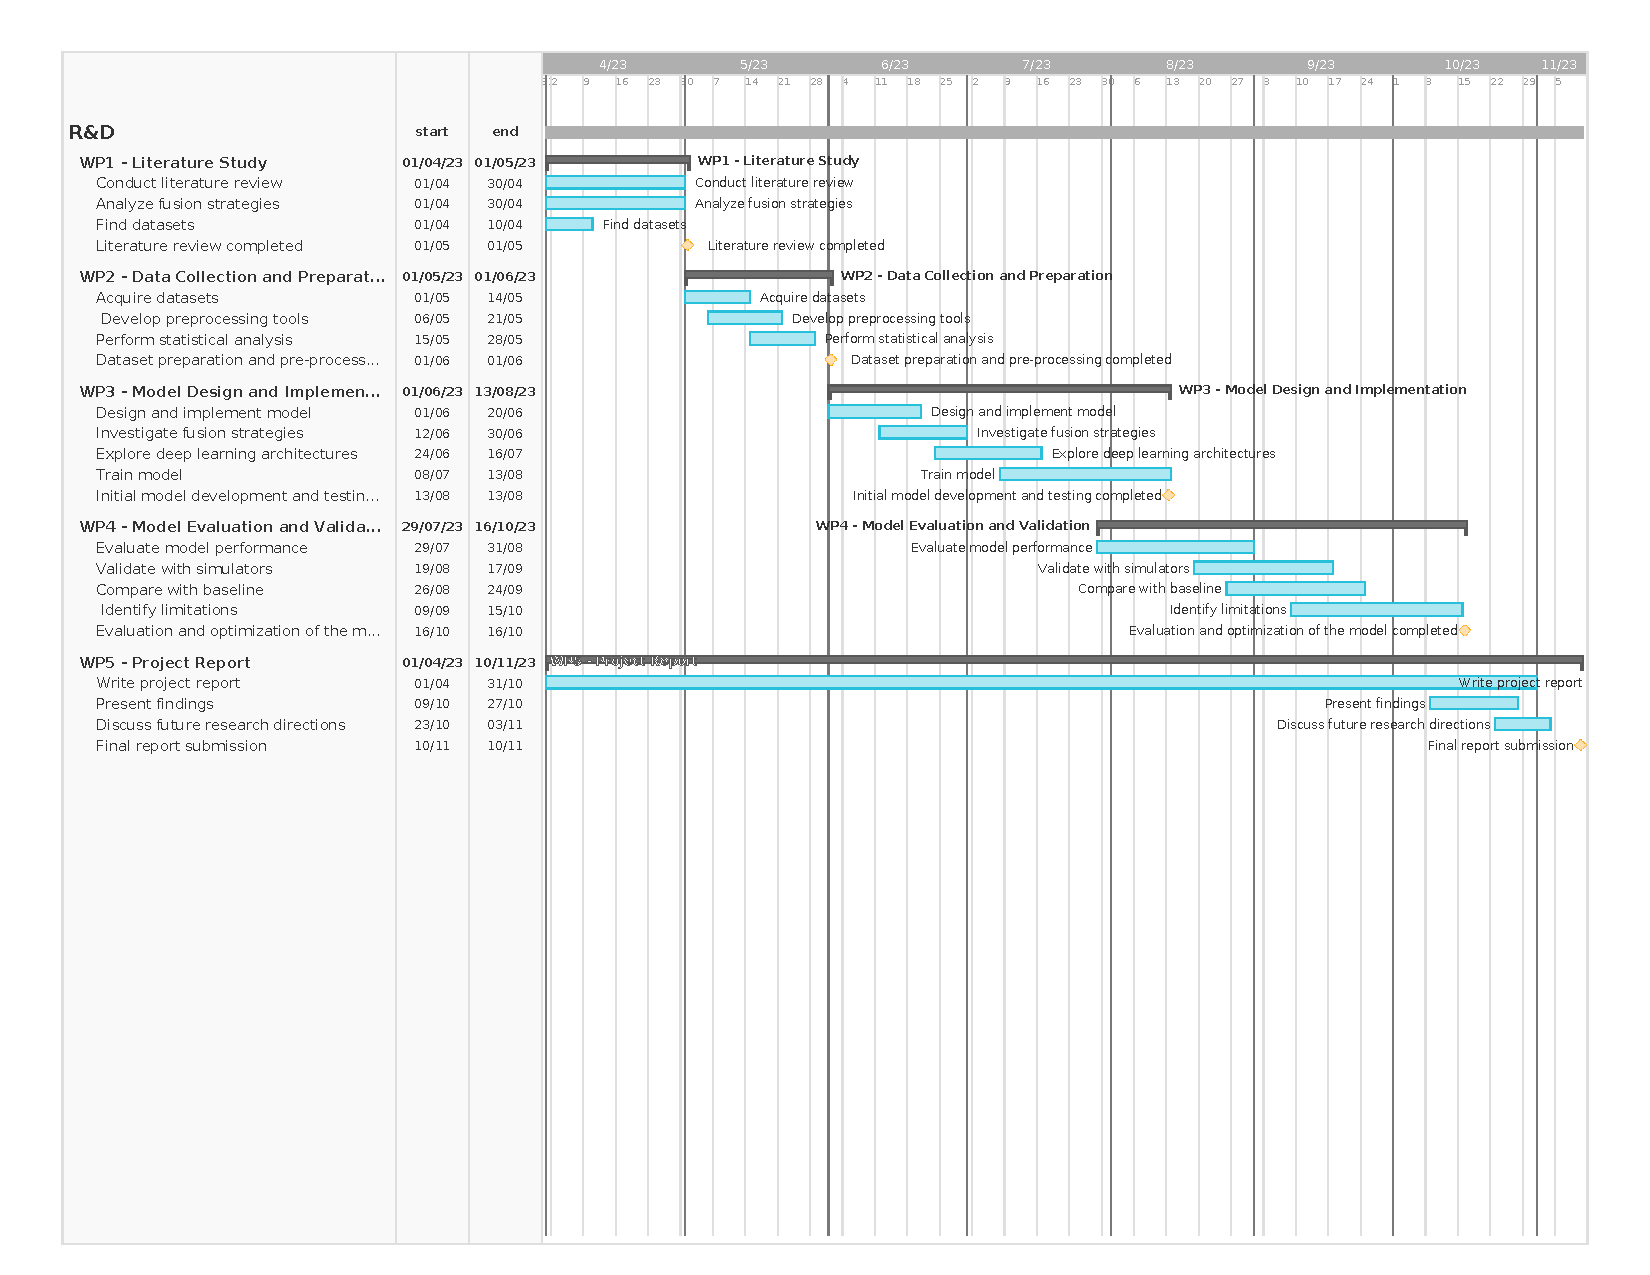
\includegraphics[scale=0.75]{images/Gantt_chart_landscape.pdf}
    \caption{Gantt chart of the project schedule}
    \label{fig:myfigure}
\end{figure}

\newpage
\subsection{Deliverables}
\subsubsection*{Minimum Viable}
\begin{itemize}
    % \item Project results required to get a satisfying or sufficient grade.
    \item Conduct a comprehensive literature review on state-of-the-art multimodal object detection methods and their fusion strategies
    \item Develop and test an initial model for object detection
    \item Perform a comparative analysis of at least two methods on two datasets
    \item Produce a project report that summarizes the work done and the results obtained
    %     \item Successfully detect a single class of objects, such as cars, pedestrians, cyclists, or trucks.
\end{itemize}

\subsubsection*{Expected}
\begin{itemize}
    % \item Project results required to get a good grade.
    \item Compare with more advance methods with baseline methods on different datasets
    \item  Complete the final development and testing of the model, including comparison with existing state-of-the-art methods and analysis of the strengths and weaknesses of each approach.
    \item Produce a more extensive project report that details the methodology, experimental setup, results, and analysis.
%     \item Successfully detect multiple classes of objects, such as cars, pedestrians, cyclists, or trucks.
\end{itemize}

\subsubsection*{Desired}
\begin{itemize}
    % \item Project results required to get an excellent grade.
%     \item Run experiments on CARLA simulator to validate the performance of a model
%     \item Implementation and testing of the models in a real-world scenario using CARLA or other simulators
    \item Conduct experiments to validate the model's performance by implementing and testing it in CARLA or other simulators
          \begin{itemize}
              \item Note: CARLA simulator doesn't support 4D radar sensor
          \end{itemize}
    \item Utilize spatial and temporal information from multimodal sensors in the object detection process

      % ############################
      % Future Work
      % \item Object tracking
      % \item 3D object detection
      % ############################

\end{itemize}

% Please note that the final grade will not only depend on the results obtained in your work, but also on how you present the results.

\nocite{*}

\bibliographystyle{unsrt} % Use the plainnat bibliography style
\bibliography{bibliography.bib} % Use the bibliography.bib file as the source of references

\end{document}